\documentclass[paper=a4,       % Papiergröße A4
			 11pt,
			 BCOR0mm,  % Bindekorrektur
			 DIV10,    % Satzspiegel mit 10er-Teilung
			 automark, % lebende Kolumnentitel
			 twoside,
			 halfparskip,
			 bibtotoc,
			 headsepline,
			 normalheadings,
			 appendixprefix,
			 pagesize  % Seitengröße wird bei dvi und pdf richtig gesetzt
 ]{scrbook}
\setcounter{secnumdepth}{4}
\setcounter{tocdepth}{4}
% gängige Standardpakete
\usepackage[english]{babel}
\usepackage{graphicx}
\usepackage{microtype}
\usepackage{url}
\usepackage{mparhack, fixltx2e, ellipsis} % JW: diverse Bugfixes
\usepackage{colortbl, longtable, tabularx, lscape} %JW: farbige Tabellen, umgebrochene Tabellen, Tabellen mit Skalierung auf Seitenbreite, Querformat
\usepackage[pdftex]{xcolor} % benötigt um Schriftfarbe für Todos oder Hinweise zu ändern JW: Option hinzugefügt
\usepackage[english]{varioref} %JW: Verweise wie "Abbildung 4 auf der gegenüberliegenden Seite"


%%%%%%%%%%%% Schriften %%%%%%%%%%%%%%%%%%%%%%%%%%%%%%%%%%%%%%%%%%%%%%%%%%%%%%%%%
\usepackage[T1]{fontenc}				% T1-Schriften verwenden
\usepackage[utf8]{inputenc}

%Schriftart = Palatino
\usepackage{mathpazo}
\usepackage[scaled=0.9]{helvet}
%\usepackage[scaled=0.885]{luximono}		% TeleType-Schrift: Luxi Mono

\usepackage{setspace}					% 1.05-facher Zeilenabstand wegen Palatino
\linespread{1.02}

%%%%%%%%%%%% Schriften %%%%%%%%%%%%%%%%%%%%%%%%%%%%%%%%%%%%%%%%%%%%%%%%%%%%%%%%%
%Package A4wide, um den Platz auf einem A4 Papier besser auszunutzen   
\usepackage{a4wide} %JW: Dieses Paket widerspricht jeglicher Regel für schöne Typografie

%Package Booktabs für "`schönere"' Tabellen
\usepackage{booktabs}

%Paket Listings für "`schöne"' Code-Umgebungen
\usepackage{listings}

\usepackage{rotating}

\usepackage{placeins}

\usepackage{subfigure}

\usepackage[htt]{hyphenat}

\usepackage{array}

\usepackage[printonlyused]{acronym}

\usepackage[pass]{geometry}

\usepackage{mathtools}

\usepackage{algpseudocode}

\usepackage[toc,page]{appendix}


\usepackage{url}\usepackage{url}\usepackage{url}

%Paket Caption zur Formatierung von Tabellen- und Bildunterschriften 
\usepackage[margin=25pt,font=small,labelfont=bf, format=hang]{caption}

%Paket Hyperref für den pdf-Export
\usepackage[pdfpagelabels]{hyperref}
\hypersetup
	{%
	pdftitle = {Master Thesis Report},
	pdfsubject = {Context-based Manufacturing Process},
	pdfauthor = {Debasis Kar},
	pdfkeywords = {Industry 4.0, Manufacturing, IoT, BPMN, Internet of Things, CPS, Cloud, Business Pocess Modeling, Smart Factory},
	colorlinks = {true},
	citecolor = {black},
	linkcolor = {black},
	urlcolor  = {black},
	a4paper
	}

% Package ntheorem für Definitionen, Sätze, etc.
\usepackage[standard,hyperref]{ntheorem}
\newtheorem{Def}{Definition}[chapter]
\newtheorem{Begriff}{Term}[chapter]

%----------------  Kopf- und Fußzeilen  --------------------------------------
\usepackage{scrpage2}
\pagestyle{scrheadings}

\cfoot[]{}
\ifoot[]{}
\ofoot[\pagemark]{\pagemark}
\ohead[]{}
\chead[]{}
\ihead{\headmark}
%-----------------------------------------------------------------------------

%%%%%%%%%%%%%%%%%%%%%%%%%%%%%%%%%%%%%%%%%%%
%Änderung der Kapitelüberschriften
%%%%%%%%%%%%%%%%%%%%%%%%%%%%%%%%%%%%%%%%%%%

%-----------------------------------------------------------------------------
\renewcommand*{\chapterheadstartvskip}{}
%-----------------------------------------------------------------------------

\newcommand*{\ORIGchapterheadstartvskip}{}
\let\ORIGchapterheadstartvskip\chapterheadstartvskip
 \renewcommand*{\chapterheadstartvskip}{
   \ORIGchapterheadstartvskip
   {
     \setlength{\parskip}{0pt}
     \noindent\rule[.3\baselineskip]{\linewidth}{1pt}
   }
 }
\newcommand*{\ORIGchapterheadendvskip}{}
\let\ORIGchapterheadendvskip\chapterheadendvskip
\renewcommand*{\chapterheadendvskip}{
{
\setlength{\parskip}{0pt}
\noindent\rule[.3\baselineskip]{\linewidth}{1pt}\par
}
\ORIGchapterheadendvskip
}
%%%%%%%%%%%%%%%%%%%%%%%%%%%%%%%%%%%%%%%%%%%
%Ende Änderung der Kapitelüberschriften
%%%%%%%%%%%%%%%%%%%%%%%%%%%%%%%%%%%%%%%%%%%

%Trennungsliste
\hyphenation{}

%%%%%%% Custom Commands %%%%%%%%%%%%%%%%%%%%%%%%%%%%%%%%%%%%%%%%%%%%%%%%%%%%%%%%

\newcommand{\term}[1]{\textit{#1}}
\newcommand{\code}[1]{\texttt{#1}}
\newcommand{\refsection}[1]{(see~Sect.~\ref{#1})}
\newcommand{\refappendix}[1]{(see~Appendix~\ref{#1})}
\newcommand{\reflisting}[1]{(see~Listing~\ref{#1})}
\newcommand{\reffig}[1]{(see~Fig.~\ref{#1})}
\newcommand{\reftable}[1]{(see~Table~\ref{#1})}

\newcommand{\acrodep}[2]{\acro{#1}{#2 \acroextra{ \textit{(deprecated)}}}\acused{#1}}

%%%%%%% Listings %%%%%%%%%%%%%%%%%%%%%%%%%%%%%%%%%%%%%%%%%%%%%%%%%%%%%%%%%%%%%%%

%Setzen der Einstellungen für das Listings-Paket am Beispiel Java
%\definecolor{comments-eclipse-style}{rgb}{0.25,0.5,0.37}
%\definecolor{keywords-eclipse-style}{rgb}{0.5,0.0,0.33}
%\definecolor{strings-eclipse-style}{rgb}{0.16,0.0,1.0}

% JW: Beachte, dass jede farbige Seite Geld kostet oder im Ausdruck anders rüberkommt. Ich hab alles schwarz-weiß gemacht. Außerdem helfen Nummerierungen für Verweise. Kommentiere den Stil aus, der Dir mehr zusagt.
\definecolor{comments-eclipse-style}{rgb}{0.5,0.5,0.5}
\definecolor{keywords-eclipse-style}{rgb}{0.35,0.35,0.35}
\definecolor{strings-eclipse-style}{rgb}{0.0,0.0,0.0}

\newcommand\myKeywordStyle{\bfseries}

\definecolor{black}{rgb}{0.0,0.0,0.0}

\lstset{%
	basicstyle=\ttfamily,
	numbers=left,
	numberstyle=\tiny,
	stepnumber=1,
	numbersep=10pt,
	frame=tb,
	framerule=\heavyrulewidth,
	tabsize=2,
	captionpos=b,
	breaklines=true,
    breakatwhitespace=false,
    aboveskip=1.5em,
    belowskip=1em,
	keywordstyle=\color{keywords-eclipse-style},
	commentstyle=\color{comments-eclipse-style},
	stringstyle=\color{strings-eclipse-style}
}

%JW: Original
%\lstdefinestyle{java}
%	{language=Java,
%	 basicstyle=\ttfamily,
%	 identifierstyle=\ttfamily,
%	 keywordstyle=\color{keywords-eclipse-style},
%	 commentstyle=\color{comments-eclipse-style},
%	 stringstyle=\color{strings-eclipse-style},
%	 %numbers=left,
%	 %numberstyle=\tiny,
%	 %stepnumber=1,
%	 %numbersep=10pt,
%	 frame=single,
%	 captionpos=b
%}

%\lstdefinestyle{xml}
%	{language=XML,	 
%	 basicstyle=\ttfamily,
%	 identifierstyle=\ttfamily,
%	 keywordstyle=\color{keywords-eclipse-style},
%	 commentstyle=\color{comments-eclipse-style},
%	 stringstyle=\color{strings-eclipse-style},	 
%	 captionpos=b,
%	 showstringspaces=false
%}

%\lstdefinestyle{xml}
%	{language=XML,	 
%	 basicstyle=\ttfamily \small,
%	 captionpos=b,
%	 showstringspaces=false
%}
%
\lstdefinestyle{Java}
	{language=Java,	 	 
	 basicstyle=\ttfamily \footnotesize
}
\lstdefinestyle{xml}
	{language=XML,	 	 
	 basicstyle=\ttfamily \footnotesize
}
\lstdefinelanguage{EBNF} {
	morecomment=[s]{/*}{*/},
	morestring=[b]"
}
\lstdefinestyle{ebnf}
	{language=EBNF,	 	 
	 basicstyle=\ttfamily \footnotesize,
	 stringstyle=\color{keywords-eclipse-style}
}
%%%%%%% Ende Listings %%%%%%%%%%%%%%%%%%%%%%%%%%%%%%%%%%%%%%%%%%%%%%%%%%%%%%%%%%


%Chapter-Überschriften linksbündig
\renewcommand*{\chapterformat}{%
\chapappifchapterprefix{\ \hspace{0.75cm}}
\makebox[5pt][r]{\thechapter\autodot\enskip}}

%%% Intelligente Querverweise (Verwendung siehe meine Arbeit) %%%%%%%%%%%%%%%%%%
%% Copied from the TeXbook
\newcommand \jwIfundefined[1]{%
\expandafter\ifx\csname#1\endcsname\relax}

\newcommand \myRefRange[3]{%
\newcount\myCounter
\myCounter=#3
\advance \myCounter by -#2%
\advance \myCounter by -1 %
\ifnum \myCounter=0\relax
	\ref{#1} auf Seite~#2\,f.%
\else
	{\ref{#1} auf Seite~#2\ bis~\pageref{#1:end}}%
\fi
}

\newcommand \myRefi[1]{%
\jwIfundefined{r@#1:end}{\vref{#1}}\else
{% 3 Fälle:
%  - nur eine Seite: kein Bereich, sondern wie \vref
%  - 2 Seiten -> f
%  - > 2 Seiten: Bereich
\vrefpagenum\jwFirstnum{#1}%
\vrefpagenum\jwSecondnum{#1:end}%
%
\ifthenelse{\equal\jwFirstnum\jwSecondnum}%
{\vref{#1}}% Fall 1
{\myRefRange{#1}\jwFirstnum\jwSecondnum}% Secondnum >= firstnum + 1
}\fi
}

\newcommand\myVref[1]{%
\jwIfundefined{r@#1}{\vref{#1}}\else
{\myRefi{#1}}\fi
}

%%%%%%%%%%%%%%%%%%%%%%%%%%%%%%%%%%%%%%%%%%%%%%%%%%%%%%%%%%%%%%%%%%%%%%%%%%%%%%%%

\begin{document}
%%%%%%%%%%%%%%%%%%%%%%%%%%%%%%%%%%%%%%%%%%%
%Erzeugung des Titelblatts
%%%%%%%%%%%%%%%%%%%%%%%%%%%%%%%%%%%%%%%%%%%
% Deckblatt zentrieren
%\newlength\oddsidemarginorig
%\oddsidemarginorig=\oddsidemargin
%\oddsidemargin 1.05cm
%\newgeometry{a4paper,left=20.05mm,right=10mm, top=29.7mm, bottom=29.7mm}
%\thispagestyle{plain}
\pagestyle{plain}
\begin{titlepage}
\begin{sffamily}
\begin{center}
Institute of Architecture of Application Systems\\
University of Stuttgart\\
Universitätsstraße 38\\
D-70569 Stuttgart\\
\end{center}

\vspace{3.0cm}

\begin{center}
{Master Thesis No. ---}\\
\vspace{0.5cm}
\begin{minipage}{8.5cm}
\begin{center}
 
  \Large \textbf{Context-based Manufacturing Processes}
 
\end{center}
\end{minipage}
\\
\vspace{1cm}
{Debasis Kar}
\end{center}

\vspace{1.0cm}

\begin{center}
\begin{minipage}{3cm}
\begin{center}
	
\includegraphics[width=0.9\textwidth]{./gfx/unilogo.pdf}
	%\includegraphics{./gfx/uni_logo.png}
\end{center}
\end{minipage}
\begin{minipage}{3cm}
\begin{center}
	
\includegraphics{./gfx/iaas.jpg}
\end{center}
\end{minipage}
\end{center}
%
\vspace{1.0cm}
%
\begin{center}
\begin{tabular}{ll}
\textbf{Course of Study:} & M.Sc. INFOTECH\\
&\\&\\
\textbf{Examiner:} & Prof. Dr. Dr. h. c. Frank Leymann\\
&\\
\textbf{Supervisor:} & M.Sc. C. Timurhan Sungur\\
&\\                     
\textbf{Commenced:} & September 09, 2015\\
&\\
\textbf{Completed:} & March 09, 2016\\
&\\
\textbf{CR-Classification:} & H.4.1, J.7, K.1\\

\end{tabular}
\end{center}
\end{sffamily}
\end{titlepage}
%\oddsidemargin=\oddsidemarginorig
\restoregeometry
%%%%%%%%%%%%%%%%%%%%%%%%%%%%%%%%%%%%%%%%%%%
%Ende Titelblatt
%%%%%%%%%%%%%%%%%%%%%%%%%%%%%%%%%%%%%%%%%%%
\cleardoubleemptypage

\setlength{\parindent}{0.0em}

\pagenumbering{roman}

\begin{center}
\section*{Abstract}
\end{center}
\pagestyle{empty}
--- Abstract comes here ---

\cleardoubleemptypage
\pagestyle{scrheadings}
\tableofcontents
\newpage
\let\cleardoublepage\clearpage

\listoffigures
\let\cleardoublepage\clearpage
\let\cleardoublepage\relax
\listoftables
\let\cleardoublepage\clearpage
\renewcommand{\lstlistlistingname}{List of Listings}
\lstlistoflistings
\let\cleardoublepage\clearpage
\cleardoubleemptypage

%\sloppy

\pagenumbering{arabic}
\newpage
\chapter{Introduction} \label{chap:introduction}Economists assert manufacturing to be a wealth-producing sector of an economy, since manufacturing process involve the processes to transform raw materials into finished goods on a large scale. Manufacturing world thrives upon many complex variables. In the recent years, due to innovations in \acs{ICT} the focus of supply and demand are shifting, thus manufacturing industry is experiencing complex supply chains. Customers demanding high levels of individualized products are driving fierce competition in pricing and forcing manufacturers to strive for highest levels of efficiencies. Still manufacturers can develop effective survival strategies amidst all these turbulences \reffig{fig:1.1} if they are able to continuously adapt their organizational structures \cite{WESTKAMP}.

The challenge for adaptive manufacturing is to access all available information when it is needed, where it is needed, and in the form it is most useful to drive optimal actions and responses \refsection{IOT}. Adaptive manufacturing also enables manufacturers to generate and apply data-driven manufacturing intelligence throughout the life-cycle of design, engineering, planning and production.

A new wave of technological changes \refsection{ind4} is already driving a paradigm shift in manufacturing. Manufacturing sector is at the verge of a new industrial revolution which promises all range of opportunities for innovation in terms of smarter industrial processes, new business models and customized products. The new technological wave builds on the concept of interaction between the real and virtual worlds which becomes the core of the manufacturing processes. Both production equipment and manufactured products are now able to gather, process and analyze data of the physical world and interact with each other autonomously.
\begin{figure}[h!]
	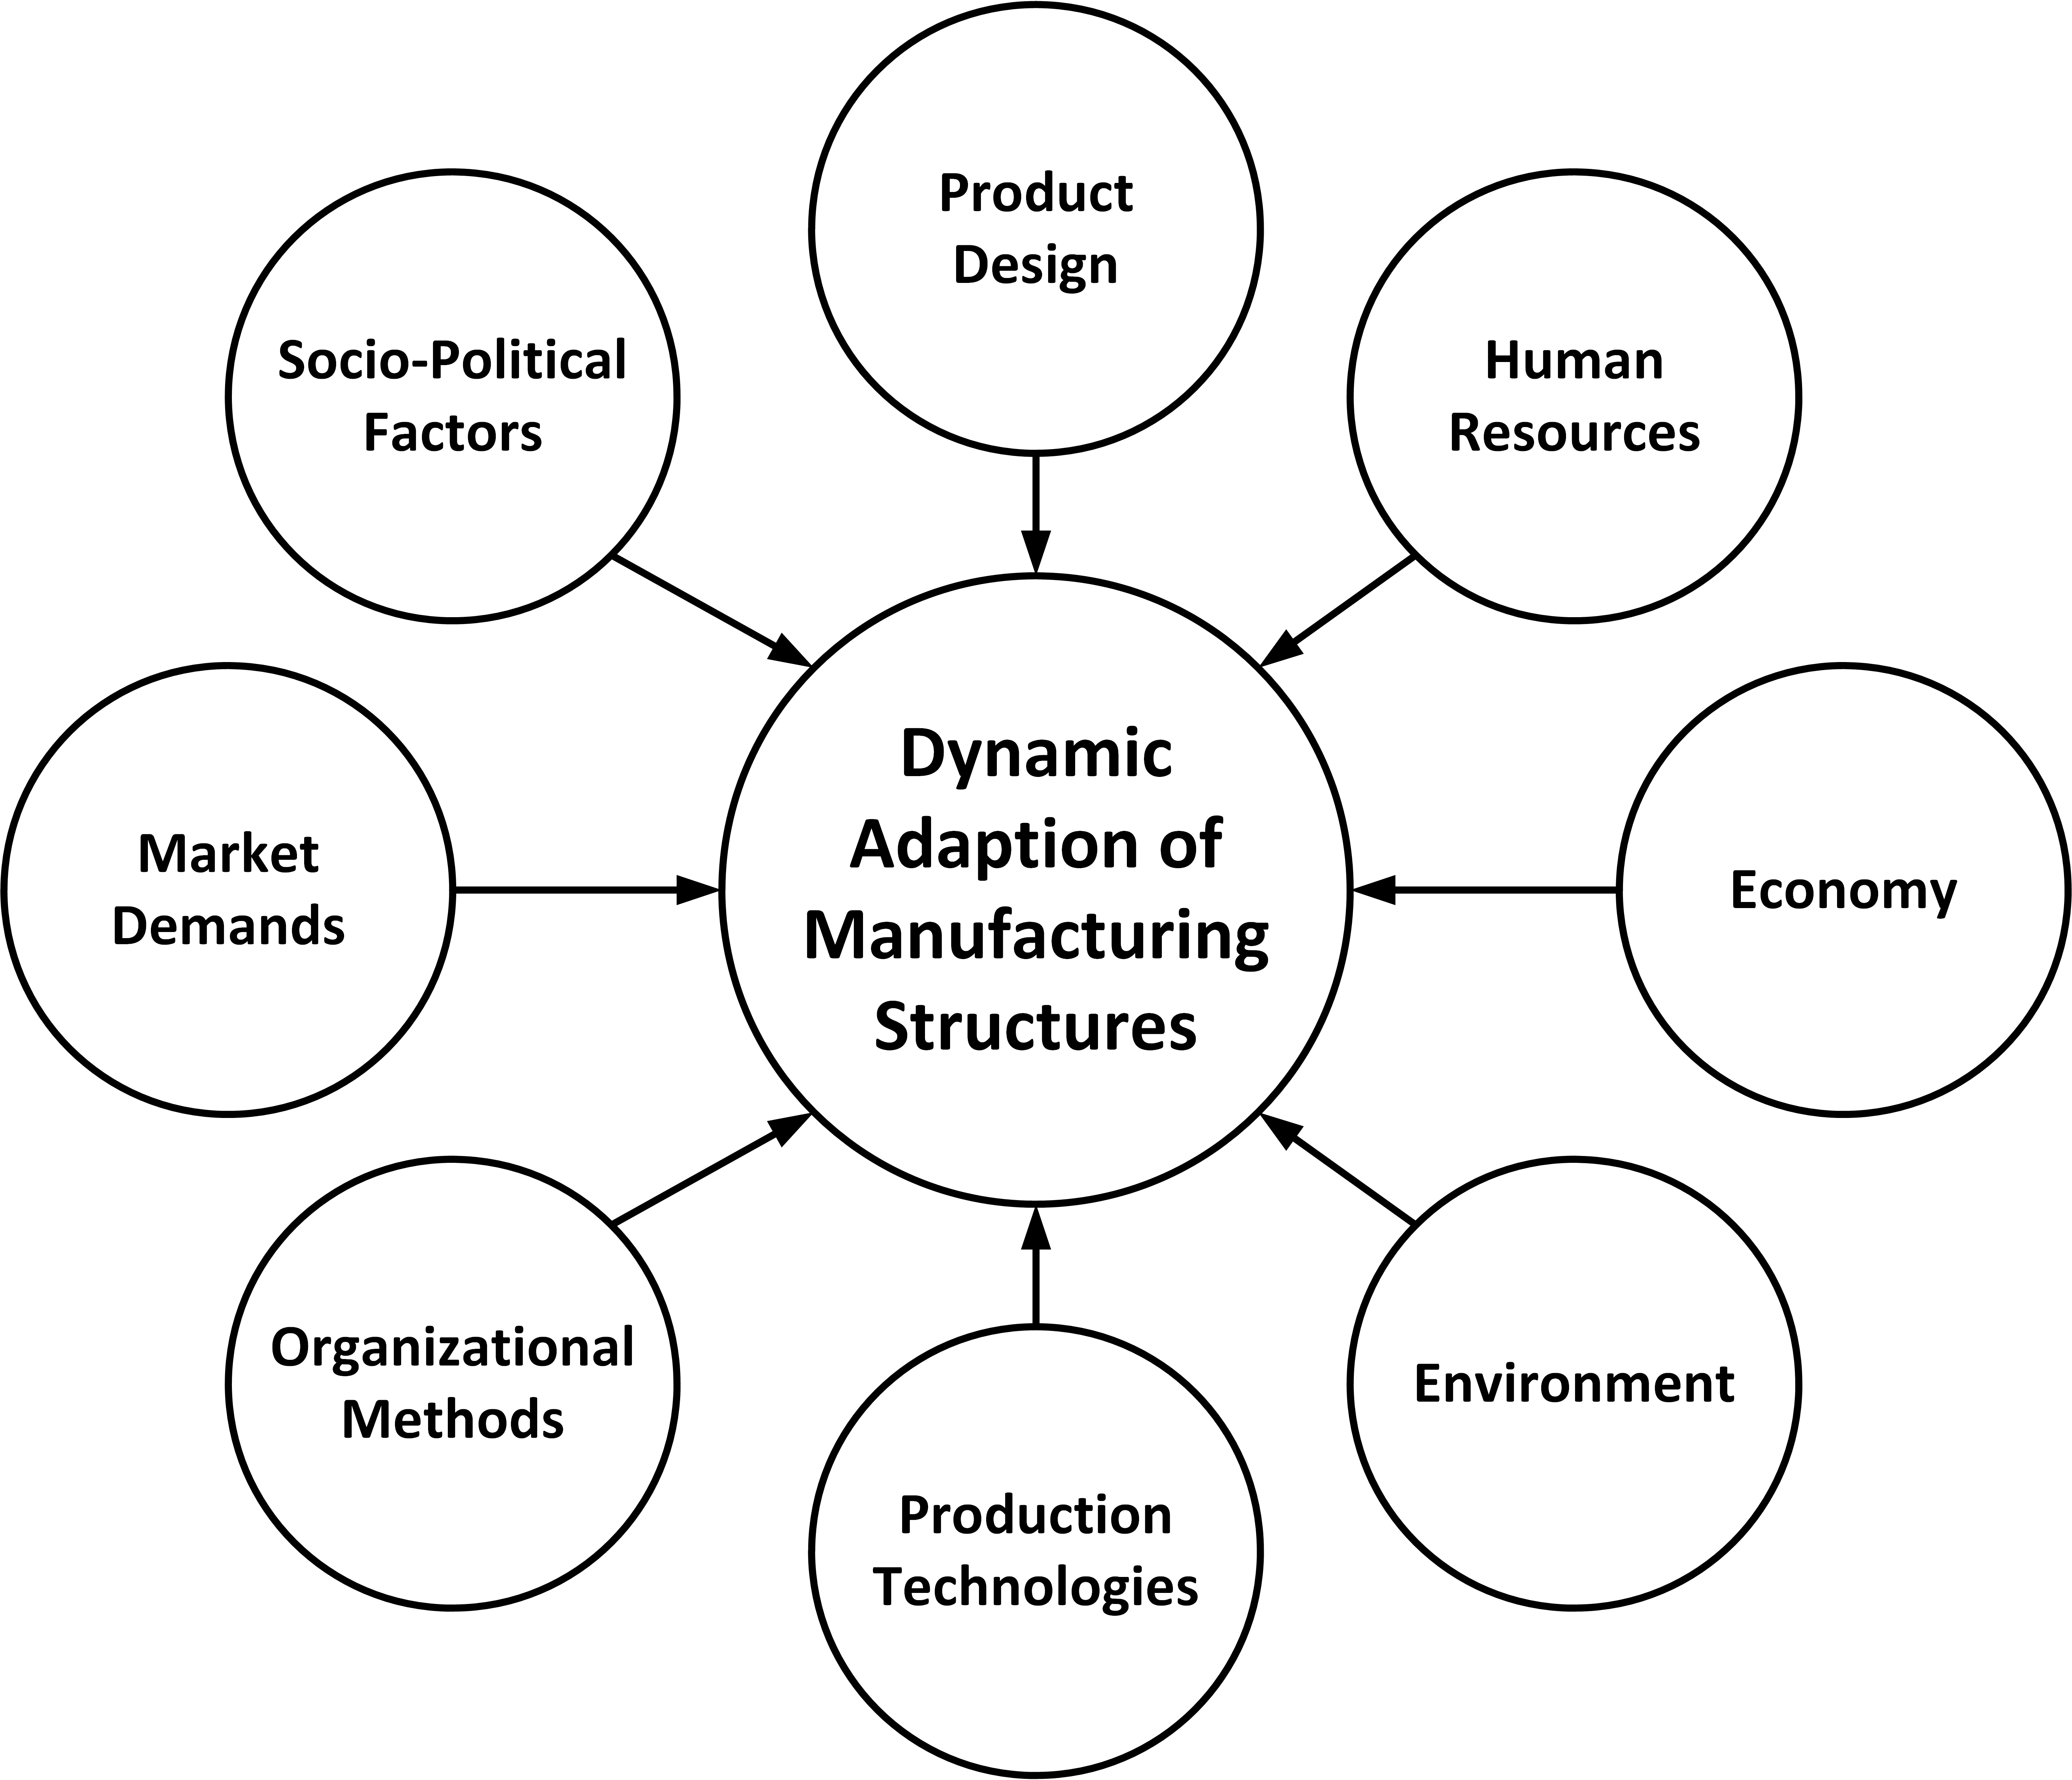
\includegraphics[scale=0.4]{./gfx/addmanustr}
	\centering
	\caption{Adapting the Structures of Manufacturing \cite{WESTKAMP}}
	\label{fig:1.1}
\end{figure}

To increase the efficiency of production process, automation, optimization, and dynamic adaption became the most important requirements in manufacturing sector. Since the dawn of sensors and networking technologies \refsection{IOT} vital information can be gathered before-hand to decide the most suitable and optimized process.  The selection of each execution step may depend on different factors as new technological advancements provide more solution options to the same kind of problems. Manually conducted assembly tasks may provide alternatives to the existing automation methods depending on the current demand, status of the machinery, and occupation of the machinery \cite{TIMURCIRP}. Situations can be observed using smart-systems \refsection{CPS} which enable the application of well-adopted business process modeling and execution  solutions in the context of manufacturing companies and tracking of activity flows in the real world \cite{CONWORKFLOW}.

Production or Manufacturing processes can be modeled using business process process modeling languages e.g. the Business Process Execution Language (\acs{BPEL}) \cite{BPELSPEC} or the Business Process Model and Notation (\acs{BPMN}) \cite{OMGSPEC}. After modeling, the process models are deployed on compliant work-flow engines for an automated execution. But these paradigms don not support adaptive and flexible execution of business processes in manufacturing sector. By not considering these adaptations, the manufacturing companies lose their revenue and edge in market by remaining reluctant to structural changes on time \cite{TIMURCIRP,CONWORKFLOW}.
\section{Problem Statement}
Manufacturing processes need to be updated regularly to stay competitive in the market was the theme of last section. With the emergence of Internet of Things \refsection{IOT}, the manufacturing processes can be made smarter to leverage the next industrial revolution - Industry 4.0 \refsection{ind4}.

Sungur et al. \cite{TIMURCIRP} presented a novel approach to support \textit{Context-sensitive Adaptive Production Process} in their research work. They extended production processes, which contain a sequence of predefined sets of sub-processes, with \textit{Context-sensitive Execution Steps (\acs{CES})} \refsection{conces}. For each \acs{CES}, context-relevant sub-processes are chosen and desired processes are elected, optimized, deployed and executed \cite{TIMURCIRP}.

\acs{CES} approach dictates a way in which processes can possibly adapt themselves to the execution context. In each context, there can be multiple alternatives for the same process goals and the best needs to be selected and executed at runtime \cite{TIMURCIRP}.
\section{Scope of Work}
\chapter{Fundamentals} \label{chap:fundamentals}
For much of human history, productivity growth was barely perceptible, and living standards improved at a snail's pace. Then approximately 200 years ago, a steep change in innovation occurred: the \textit{Industrial Revolution} treated as \textit{Industry 1.0}, in which the muscle power of all living beings was replaced by mechanical power that introduced steam engines and internal combustion engines to the mechanical production facilities. From the early part of the twentieth century, electrification and the division of labor led to the second industrial revolution which is referred as \textit{Industry 2.0} now. The third industrial revolution referred as \textit{Industry 3.0}, also known as the \textit{Digital Revolution}, was set in around the 1970s, when advanced electronics and \acs{IT} developed further the automation of production processes. In the following decades industrial technological advancements were only incremental, especially compared with the breakthroughs that transformed \acs{IT}, mobile communications, and e-commerce \cite{INDUSINTERNET,IN4DESIGN,IN4BCG}.

Productivity and economic growth accelerated sharply in consequence of these innovations. The number of manufacturing jobs decreased, new jobs emerged and the demand for new skills grew. Today, another workforce transformation is on the horizon as manufacturing experiences a new wave of technological advancement where it is possible to augment physical machines with digital intelligence. The conditions are ripe and early evidence suggests that this new wave of innovation is already upon us \cite{INDUSINTERNET,MANMACHINE}.

In the next few sections we have discussed about how the next industrial revolution will unfold itself, and its benefits for businesses and more broadly for economies around the world.
\section{Industry 4.0} \label{ind4}
The term \textit{“Industry 4.0”} that refers to the next industrial revolution became publicly known in 2011 at Hanover Fair, when an initiative named \textit{“Industrie 4.0”} - an association of representatives from business, politics, and academia - promoted the idea as an approach to strengthening the competitiveness of the German manufacturing industry \cite{VDINACH}. The German Federal Government (Die Bundesregierung der Bundesrepublik Deutschland) supported the idea by announcing that Industry 4.0 will be an integral part of its “High-Tech Strategy 2020 for Germany” initiative, aiming at technological innovation leadership. The subsequently formed “Industrie 4.0 Working Group” then developed first recommendations for implementation, which were published in April 2013 \cite{IN4DESIGN}.

Hermann et al. \cite{IN4DESIGN} describe the fascination behind Industry 4.0 in 2 segments. Firstly, for the first time an industrial revolution is predicted a-priori, not observed ex-post that provides various opportunities for companies and research institutes to actively shape the future. Secondly, Industry 4.0 promises substantially increased operational effectiveness as well as the development of entirely new business models, services and products.
\subsection{Definition}
From the literature review of Hermann et al. \cite{IN4DESIGN} and Kagermann et al. \cite{VDINACH},
\begin{definition}
\textit{Industry 4.0} is a collective term for contemporary automation, data exchange, and manufacturing technologies and concepts of value chain organization which draws together Cyber-Physical Systems (\acs{CPS}), the Internet of Things (\acs{IoT}), Smart Factories and the Internet of Services. 
\end{definition}
Rüßmann et al. \cite{IN4BCG} explain it in a similar way.
\begin{definition}
\textit{Industry 4.0} is a new digital industrial technology that will connect sensors, machines, work-pieces, and \acs{IT} systems along the value chain beyond the enterprise which in turn will interact with another using standard Internet-based protocols and adapt to changes.
\end{definition}
In North America, similar ideas have been brought up under the name \textit{Industrial Internet} by General Electric \cite{INDUSINTERNET}. The technical basis is very similar to Industry 4.0, but the application is broader than industrial production. The various definitions have caused confusion rather than increasing transparency \cite{IN4HYPE}. Hereafter Industrie 4.0 or Industrial Internet will be referred interchangeably with Industry 4.0.
\subsection{Enablers of Industry 4.0}
\begin{figure}[h!]
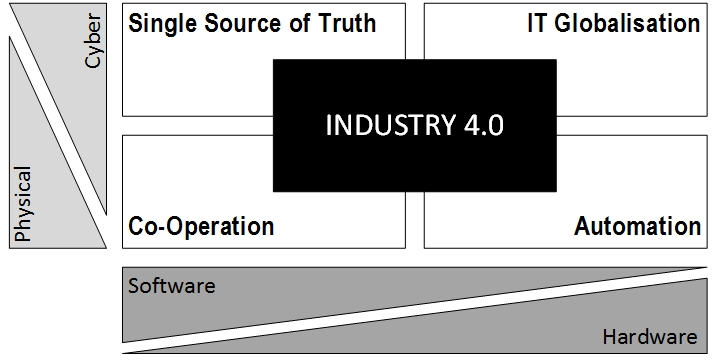
\includegraphics[scale=0.6]{./gfx/indus4enablers}
\centering
\caption{Four Enablers of Industry 4.0 - Adapted from \cite{IN4HYPO}}
\label{fig:2.1}
\end{figure}
Industry 4.0 is not initiated on a shop-floor level and therefore companies have to take measures in their own hands to introduce its enablers into their companies to profit from the current change in society and technology \cite{VDINACH}. 
These measures can be categorized by the aid of 2 dimensions. The first dimension describes whether a precondition is physical or cyber, whereas the second dimension allocates the precondition to hard- or software components. Industry 4.0 can be seen as a collaborated production by the inter-working of human-human, machine-human, and machine and production system \reffig{fig:2.1} \cite{IN4HYPO}.
\begin{itemize}
\item \textit{Single Source of Truth} dictates to embed all product life-cycle data along the value chain within a single database using cloud storage and accesses to make all changes to product and production visible and avoid ambiguity during production and simulations \cite{IN4HYPO}.
\item \textit{\acs{IT}-Globalisation} had made computers achieve exponential growth in speed and cheap storage capacity. This will allow faster extensive simulations of different aspects of a company as well as the processing of huge amounts of data, which are already collected by companies, but cannot be used adequately \cite{IN4HYPO}.
\item \textit{Automation} leads to automated and decentralized processes which can be combined to collaboration networks and are able to adapt to dynamic requirements and therefore are self-optimizing \cite{IN4HYPO}.
\item \textit{Co-Operation} aims at the connection of all technologies and activities e.g. efficient sharing and exchange of engineering data within a
network of engineers. Networks help to improve cooperation by communicating targets and empowering decision maker’s in decentralized systems \cite{IN4HYPO,VDINACH}.
\end{itemize}
\subsection{Components of Industry 4.0 Enablers}
Advances in technology that powered Industry 4.0 are already used in manufacturing, but with Industry 4.0, they will transform production: isolated cells will come together as a fully integrated, automated, and optimized production flow, leading to greater efficiencies and changing traditional production relationships among suppliers, producers, and customers — as well as between human and machine \cite{IN4BCG}. Major factors that propels this next industrial revolution has been listed below.
\begin{itemize}
\item \textit{Cyber Physical Systems (\acs{CPS})} \refsection{CPS} are integrations of computation, networking and physical processes. Embedded computers and networks monitor and control the physical processes, with feedback loops where such processes affect computations and vice versa e.g. autonomous automotive systems \cite{IN4DESIGN}.
\item \textit{Internet of Things (\acs{IoT})} \refsection{IOT} allows field devices to communicate and interact both with one another and with more centralized controllers, as necessary. It also decentralizes analytics and decision making, enabling real-time responses \cite{IN4BCG,IN4DESIGN}.
\item \textit{Smart Factory} is context-aware by assisting people and machines in execution of their tasks. It is achieved by systems working in background, so-called Calm-systems and context aware means that the system can take into consideration information coming 	from physical and virtual world like the position and status of an object \cite{IN4DESIGN}.
\item \textit{Internet of Services (\acs{IoS})} enables service vendors to offer their services via the internet. The \acs{IoS} consists of participants, an infrastructure for services, business models, and the services themselves. Services are offered and combined as value-added services by various suppliers; they are communicated to users as well as consumers and are accessed by them via various channels \cite{IN4DESIGN}.
\item \textit{Big Data and Analytics} based on large data sets has emerged only recently in the manufacturing world, where it optimizes production quality, saves energy, and improves equipment service. Big data is high volume, high velocity, and/or high variety information assets that require new forms of processing to enable enhanced decision making, insight discovery and process optimization \cite{BIGDATA}. In an Industry 4.0 context, the collection and comprehensive evaluation of data from many different sources - production equipment and systems as well as enterprise- and customer-management systems - will become standard to support real-time decision making \cite{IN4BCG,IN4DESIGN}.
\item \textit{Cloud Computing} is a model for enabling ubiquitous, convenient, on-demand network access to a shared pool of configurable computing resources (e.g. networks, servers, storage, applications, and services) that can be rapidly provisioned and released with minimal management effort or service provider interaction as per definition of \acs{NIST} \cite{MELLNIST}. It will make increased data sharing across sites and company boundaries possible for Industry 4.0. At the same time, the performance of cloud technologies will improve, achieving reaction times of just several milliseconds. As a result, machine data and functionality will increasingly be deployed to the cloud, enabling more data-driven services for production systems \cite{IN4BCG,IN4DESIGN}.
\item \textit{Augmented Reality} based systems support a variety of services, such as selecting parts in a warehouse and sending repair instructions over mobile devices. These systems are currently in their infancy, but in the future, companies will make much broader use of augmented reality to provide workers with real-time information to improve decision making and work procedures \cite{IN4BCG}.
\end{itemize}
\subsection{Mechanisms to Increase Productivity}
The significant increase of the productivity due to Industry 4.0 can be represented by the 4 mechanisms. Schuh et al. \cite{IN4HYPO} had discussed in their article how enablers of Industry 4.0 facilitate these mechanisms.
\begin{enumerate}
\item \textit{Revolutionary Product Life-cycles}: Integrated technologies
and rapid prototyping facilitate companies to produce testable prototypes which
supply viable information of the products potentials as customer feedback can be
implemented immediately. Due to the new developments in \acs{ICT} the costs of an iteration and the resulting changes are not as cost intensive as before and therefore lead to a new development process in terms of time and profit \reffig{fig:2.2} \cite{IN4HYPO}.
\begin{figure}[h!]
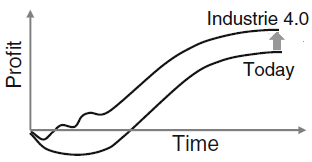
\includegraphics[scale=0.5]{./gfx/revlifecycle}
\centering
\caption{Revolutionary Product Life-cycles \cite{IN4HYPO}}
\label{fig:2.2}
\end{figure}
\item \textit{Virtual Engineering of Complete Value Chains}: By the aid of Software tools companies now have the opportunity to simulate their whole production network. This virtualization and simulation can reveal possible capacity problems as well as problems within the general work-flow. By simulating the value
chain in a short amount of time one is able to counteract possible problems before
they arise, which enhances the decision capability. To get a valuable decision capability based on simulations	it is necessary to execute an adequate number of simulations \reffig{fig:2.3} \cite{IN4HYPO}.
\begin{figure}[h!]
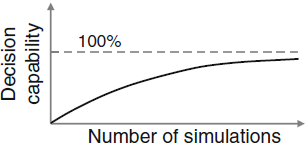
\includegraphics[scale=0.5]{./gfx/revsimul}
\centering
\caption{Virtual Engineering of Complete Value Chains \cite{IN4HYPO}}
\label{fig:2.3}
\end{figure}
\item \textit{Revolutionary Short Value Chains}: Companies have to offer more and more individualized products in order to meet the customer requirements. This complicates the division of labor introduced by Taylorism as machines in general are only able to accomplish one specific task. In order to allow even more individualized products the integration of production steps and thus the integration of functions within production systems is inevitable. This leads to a reversion of Taylorism - instead of the division of labor by means	of a conveyor belt production cells are to be established, allowing an employee to take over autonomous responsibility and give this specific employee decision \cite{IN4HYPO}. 
\begin{figure}[h!]
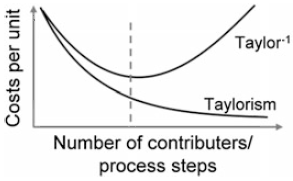
\includegraphics[scale=0.5]{./gfx/revvalchain}
\centering
\caption{Revolutionary Short Value Chains \cite{IN4HYPO}}
\label{fig:2.4}
\end{figure}

Within a production process for highly customized products there is an optimal number of contributors or process steps in one production cell which have to collaborate in order to achieve minimal costs for the produced product \reffig{fig:2.4} \cite{IN4HYPO}.
\item \textit{Better Performing than Engineered}: Companies must aim at the self-optimizing	capabilities of production systems which are already theoretically possible. With the ongoing advancement of self-optimizing production systems machines should be able to reach a productivity level which exceeds the previously determined maximum due to cybernetic effects \reffig{fig:2.5}. An example would be a productivity of 15,000 units whereas the estimated maximum before self-optimization was 10,000 units \cite{IN4HYPO}.
\begin{figure}[h!]
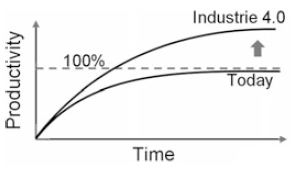
\includegraphics[scale=0.5]{./gfx/revengg}
\centering
\caption{Better Performing than Engineered \cite{IN4HYPO}}
\label{fig:2.5}
\end{figure}
\end{enumerate}
\subsection{Industrial Requirements}
For Industry 4.0, the term revolution does not refer to the technical realization but to the ability to meet today’s as well as future challenges. Some very basic requirements guide most of the work currently being done.
\begin{itemize}
\item \textit{Investment Protection}: Industry 4.0 has to be introduced stepwise into existing plants with-out hampering business and investor's trust \cite{IN4HYPE,IN4BCG}.
\item \textit{Stability}: Industry 4.0 must provide stability and must not compromise production, neither by disturbances nor by a breakdown \cite{IN4HYPE}.
\item \textit{Infrastructure Development}: Industry 4.0 will require an	adequate backbone. Data centers, broadband spectrum, and fiber networks are all components of the \acs{ICT} infrastructure that will need to be further developed to connect the various machines, systems, and networks across industries and geographies \cite{INDUSINTERNET}.
\item \textit{Data Privacy}: Access to production related data and services has to be controllable to protect company	know-how. Although	countries will develop national guidelines, the development of international norms and	standards will also be required. The focus	should be on developing norms related to IP protection and international data flows \cite{IN4HYPE,INDUSINTERNET}.
\item \textit{Cybersecurity}: Industry 4.0 has to prevent unauthorized access to production systems to prevent environmental or economic damage and harm to humans.Products	(devices and software) should contain embedded security features to maximize the layers of defense against cyber-threats \cite{IN4HYPE,INDUSINTERNET}.
\item \textit{Policymaking}: Cooperation with regulators, law enforcement, and the intelligence community can help improve the visibility of evolving threats. Courses of action include sharing threat information and mitigation efforts to build a stable foundation. The government should pursue the development and broad
adoption of voluntary industry standards and best practices for cyber-security \cite{INDUSINTERNET}.
\item \textit{Talent Development}: The rise of the Industry 4.0 will require new talent pools to be created and grown. There will be a wave of new technical,analytical, and leadership roles that are	explicitly cross-discipline e.g. Data scientists, \acs{UI} experts, Next-generation engineers etc \cite{INDUSINTERNET}.
\item \textit{Enhance Competencies}: Producers have to set priorities among their production processes and enhance their workforce’s competencies step-wise so that they can take advantage of Industry 4.0 in coming years \cite{MANMACHINE}.
\item \textit{Leverage Technologies}: Manufacturing-system suppliers need to understand how they can employ technologies in new use cases to offer the greatest benefits to their customers. These technologies can be leveraged for different offerings, such as the enhancement of networked embedded systems and automation, the development of new software products, and the delivery of new services, such as analytics-driven services \cite{MANMACHINE,INDUSINTERNET}.
\end{itemize}
Any future Industry 4.0 architecture has to fulfill these requirements as reconditions for industrial acceptance.
\subsection{Benefits of Industry 4.0 in Manufacturing}
Industry 4.0 promises to have a range of benefits spanning machines, facilities, fleets and industrial networks, which in turn influence the broader economy. Industry 4.0 opens the door to a variety of benefits for the industrial economy. Some companies have been early adopters, realizing benefits and overcoming challenges related to capturing and manipulating data streams. While its benefits would reverberate throughout the economy, the initial impact of the Industrial Internet is likely to be felt especially strongly in the area of advanced manufacturing \cite{INDUSINTERNET}.

Lorenz et al. \cite{MANMACHINE} analyzed how the industrial workforce will evolve with Industry 4.0 by looking at the effects that these new technologies will have on Germany’s manufacturing landscape, which is among the world’s most advanced. 
\begin{itemize}
\item Manufacturers will be able to increase their competitiveness, which will enable them to expand their industrial workforce at the same time that productivity increases \cite{MANMACHINE,IN4BCG}.
\item Manufacturers will be able to bring previously off-shored jobs back home as production becomes more capital intensive and the labor cost advantages of traditional low-cost locations will shrink \cite{MANMACHINE}.
\item Manufacturers will be allowed to create new jobs to meet the higher demand resulting from the growth of existing markets and the introduction of new products and services \cite{IN4BCG,INDUSINTERNET,MANMACHINE}.
\item Robot-assisted production will cause the largest net decrease in jobs in the relevant manufacturing industries, because the efficiencies it creates will allow manufacturers to significantly reduce the number of jobs on the shop floor \cite{MANMACHINE}.
\item The use of automation to assist workers with manual tasks will be particularly valuable in responding to the needs of the aging workforce in many developed countries w.g. a robot could lift a car’s interior-finishing elements, such as a roof lining, into the chassis after manual alignment by a worker \cite{MANMACHINE}.
\item Industry 4.0 will enable technology-assisted, predictive maintenance. By remotely reviewing a stream of real-time data on machine performance, the technician will be able to pro-actively identify defects and order spare parts before arriving at a site. Once on-site, the technician will be assisted in making repairs by augmented-reality technology and will be able to receive remote guidance from experts off-site. The work can also be automatically documented \cite{MANMACHINE}.
\item The machine operators will require less machine- and product-specific training but will need enhanced capabilities for utilizing digital devices and software and accessing a digital knowledge repository. Standard operating procedures for any given task will be displayed on screens or glasses such that an operator can carry out the same types of responsibilities at several machines \cite{MANMACHINE}.
\end{itemize}
Industry 4.0 creates tremendous opportunities for manufacturing industries and national economies. Although job losses will be high for some categories of work, such as assembly and production planning, job gains will be significant in other categories, particularly \acs{IT} and analytics. The extent to which Industry 4.0 ultimately promotes higher employment will depend on how successfully companies use these technological advancements to develop new products, services, and business models. Enabling companies to retrain their workforce, education systems to close the \acs{IT} skills gap, and governments to strengthen their support will be critical to realizing the promise of Industry 4.0 \cite{MANMACHINE,INDUSINTERNET}.
\section{Internet of Things} \label{IOT}
\begin{figure}[h!]
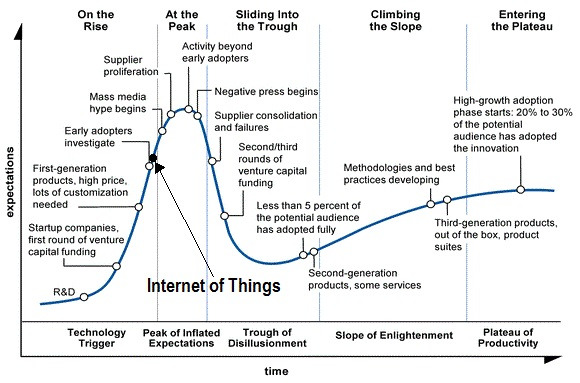
\includegraphics[scale=0.9]{./gfx/hypecycle}
\centering
\caption{\acs{IoT} in Gartner Hype-Cycle - Adapted from \cite{PICHYPECYC,HYPECYCGARTNER}}
\label{fig:2.6}
\end{figure}
The future is not going to be people talking to people; it's not going to be people accessing information. It's going to be about using machines to talk to other machines on behalf of people. We are entering a new era of ubiquity, we are entering the \acs{IoT} era in which new forms of communication between human and things, and between things themselves will be realized \cite{IOTFUTURE}. The Internet revolution led to the interconnection between people at an unprecedented scale and pace. Industry 4.0 will be the interconnection between objects to create a smart environment. Only in 2011 the number of interconnected devices on the planet overtook the actual number of people. Currently there are 9 billion interconnected devices and it is expected to reach 24 billion devices by 2020 \cite{IOTGUBBI}.

The term Internet of Things was first coined by Kevin Ashton in 1999 in the context of supply chain management \cite{IOTFIRST}. However, in recent years, the definition has been more inclusive covering wide range of applications like health-care, utilities, transport, etc.
\subsection{Definition and Trends}
\subsection{Elements of IoT}
\subsection{IoT Architecture}
\subsection{IoT and Industry 4.0}
\subsection{Cyber-Physical Systems} \label{CPS}
\subsection{IoT Augmented Manufacturing}
\section{Context-sensitive Execution Steps}\label{conces}

\chapter{Business Process Model and Notation} \label{chap:bpmn}
\section{Motivation}
\section{Reason for Selecting BPMN}
\section{Properties of BPMN}
\chapter{Motivating Scenario} \label{chap:motscene}
\chapter{Requirements for Context-Sensitive Process} \label{chap:requirements}
\chapter{Related Works and Evaluation} \label{chap:relatedworks}

% % % % Do not delete the following % % % %
\newcommand{\usecase}[8]
{
{
\small \begin{longtable}{@{}p{.2\textwidth}p{.01\textwidth}p{.79\textwidth}@{}}
\toprule Name & & \textbf{#1} \\
\midrule Goal & & #2 \\
\midrule Actor & & #3 \\
\midrule Pre-Condition & & #4 \\
\midrule Post-Condition & & #5 \\
\midrule Post-Condition in Special Case & & #6 \\
\midrule Normal Case & \multicolumn{2}{p{.8\textwidth}}{\vspace*{-0.5cm}#7} \\
\midrule Special Cases &  \multicolumn{2}{p{.8\textwidth}}{\vspace*{-0.5cm}#8} \\
\bottomrule
\caption[Description of Use Case: #1]{Description of Use Case \term{#1}.}
\end{longtable}
}
\label{table:#1}
\clearpage
}


\usecase{Enrich Topology}
{The developer wants to enrich the application topology as per the requirements.}
{Application Developer}
{The application developer has access to the winery system and has the application requirements ready.}
{Here goes the post-condition in normal case}
{Here goes the post-condition in special case}
{\begin{enumerate}
	\item Step 1 normal case
	\item Step 2 normal case
	\item ...
\end{enumerate}}
{\begin{enumerate}
	\item[1a.] Step 1a special case
		\begin{enumerate}
			\item ...
		\end{enumerate}
	\item[2a.] Step 2a special case
		\begin{enumerate}
			\item ...
		\end{enumerate}
	\item[2b.] Step 2b special case
		\begin{enumerate}
			\item ...
		\end{enumerate}
\end{enumerate}}







\chapter{Design}
\label{chap:design}


\chapter{Validation and Evaluation}
\label{chap:validationevaluation}



\chapter{Summary and Outlook} \label{chap:outcome}



\begin{appendices}
\chapter{List of Acronyms} \label{acronymlist}
	The following list contains all the acronyms which are used in this document.
		\begin{acronym}
			\acro{BPEL}{Business Process Execution Language}
			\acro{BPM}{Business Process Management}
			\acro{BPMN}{Business Process Model and Notation}
			\acro{CES}{Context-sensitive Execution Steps}
			\acro{COP}{Common Operating Picture}
			\acro{CES}{Context-sensitive Execution Step}
			\acro{CPS}{Cyber-Physical Systems}
			\acro{DFKI}{Deutsches Forschungszentrum f{\"u}r K{\"u}nstliche Intelligenz}
			\acro{DSL}{Digital Subscriber Line}
			\acro{ETSI}{European Telecommunications Standards Institute}
			\acro{EU}{European Union}
			\acro{GPRS}{General Packet Radio Service}
			\acro{IaaS}{Infrastructure as a Service}
			\acro{ICT}{Information and Communication Technology}
			\acro{IEEE}{Institute of Electrical and Electronics Engineers}
			\acro{IETF}{Internet Engineering Task Force}
			\acro{IFS}{Innovative Factory Systems}
			\acro{IoS}{Internet of Services}
			\acro{IoT}{Internet of Things}
			\acro{IP}{Internet Protocol}
			\acro{IPv6}{Internet Protocol version 6}
			\acro{ISO}{International Organization for Standardization}
			\acro{IT}{Information Technology}
			\acro{ITU}{International Telecommunication Union}
			\acro{LTE}{Long-Term Evolution}
			\acro{MEMS}{Micro-Electro-Mechanical Systems}
			\acro{NIST}{National Institute of Standards and Technology}
			\acro{OSWA}{Open Sensor Web Architecture}
			\acro{PaaS}{Platform as a Service}
			\acro{QoS}{Quality of Services}
			\acro{RFID}{Radio Frequency Identification}
			\acro{SaaS}{Software as a Service}
			\acro{SOA}{Service Oriented Architecture}
			\acro{TCP}{Transmission Control Protocol}
			\acro{UI}{User Interface}
			\acro{UMTS}{Universal Mobile Telecommunications System}
			\acro{URC}{Uniform Resource Citation}
			\acro{URL}{Uniform Resource Locator}
			\acro{URN}{Uniform Resource Name}
			\acro{WSN}{Wireless Sensor Network}
			\acro{WWW}{World-Wide Web}
%			\acro{OMG}{Object Management Group}
%			\acro{OASIS}{Organization for the Advancement of Structured Information Standards}
%			\acro{HTTP}{Hypertext Transfer Protocol}
%			\acro{REST}{Representational State Transfer}
%			\acro{SOAP}{Simple Object Access Protocol}
%			\acro{WSDL}{Web Services Description Language}
%			\acro{XML}{Extended Markup Language}
		\end{acronym}
\chapter{Glossary} \label{glossary}
The following list contains all the acronyms which are used in this document.
\end{appendices}

\bibliographystyle{alpha}
\bibliography{literatur/literatur}

All links were last followed on \today

\clearpage
\pagestyle{empty}

\pagestyle{empty}
\vspace{9cm}
\begin{center}
	\begin{minipage}{11cm}
		\vspace{6cm}
		\textbf{\Large Acknowledgement}\\\\
		\vspace{0.4cm}

		I am sincerely thankful to my mentor and supervisor C. Timurhan Sungur from the University of Stuttgart for his help, guidance, motivation and support during all the phases of my master thesis. I would also like to thank Prof. Dr. Frank Leymann for giving me this wonderful opportunity to do my master thesis at the Institute of Architecture of Application Systems.
		\vspace{0.4cm}
		 
		I am also thankful to my family and friends for their help and moral support during the tenure of my thesis.
		\vspace{1cm}
		
		Debasis Kar
	\end{minipage}
\end{center}

\pagestyle{empty}
\vspace{9cm}
\begin{center}
\begin{minipage}{11cm}
\vspace{6cm}

\textbf{\Large Declaration}\\\\
\vspace{0.4cm}

I hereby declare that the work presented in this thesis is entirely my own. 
I did not use any other sources and references that the listed ones. I have marked all direct or indirect statements from other sources contained therein as quotations. 
Neither this work nor significant parts of it were part of another examination procedure. I have not published this work in whole or in part before. 
The electronic copy is consistent with all submitted copies.
\vspace{1cm}

Stuttgart, \today \hspace{1cm}------------------------------------------\\
\phantom{Stuttgart, \today} \hspace{2.5cm} (Signature)
\end{minipage}
\end{center}
\end{document}
